\documentclass[12pt]{article}
\usepackage{amsmath, amssymb}
\usepackage{graphicx}
\usepackage{fancyhdr}
\usepackage{enumitem}
\usepackage{multicol}
\usepackage{tikz}
\usetikzlibrary{arrows}
\usepackage{geometry}
\geometry{margin=1in}

\pagestyle{fancy}
\fancyhf{}
\rhead{Devi Rosa Aprilla}
\lhead{Assignment}
\cfoot{\thepage}

\begin{document}

\begin{center}
    {Evaluasi Tengah Semester 2025} \\
    \textit{Matematika Diskrit} \\
\end{center}

\vspace{0.5cm}

\begin{center}
    {KERJAKAN MAKSIMUM 5 SOAL DARI 6 SOAL YANG DIBERIKAN!}
\end{center}

\begin{enumerate}
\item Diberikan $A = \{n \in \mathbb{N} : n \geq 2 \text{ dan } n = 4j - 5 \text{ untuk beberapa } j \in \mathbb{N}\}$ dan $B = \{n \in \mathbb{N} : n \geq 0 \text{ dan } n = 2k + 1 \text{ untuk beberapa } k \in \mathbb{N}\}$. $\mathbb{N}$ merupakan himpunan bilangan asli, atau himpunan bilangan bulat non-negatif $\{0, 1, 2, 3, 4, \ldots\}$. Buktikan bahwa $A \subset B$.

\item Dengan induksi matematika, buktikan bahwa: $57$ membagi habis $7^{n+2} + 8^{2n+1}$ jika $n$ adalah sebuah integer non-negatif.

\item Dengan induksi matematika, buktikan bahwa untuk setiap integer positif $n > 1$ berlaku
$$\frac{1}{\sqrt{1}} + \frac{1}{\sqrt{2}} + \frac{1}{\sqrt{3}} + \cdots + \frac{1}{\sqrt{n}} > \sqrt{n}$$

\item Diberikan himpunan $A = \{1, 2, 3\}$ dan $B = \{a, b, c, d\}$. Sebuah relasi $\mathbf{R}$ didefinisikan dari himpunan $A$ ke $B$ dengan aturan $R = \{(1, a), (2, b), (3, c), (3, d)\}$.
\begin{enumerate}
\item Gambarkan relasi $\mathbf{R}$ dalam bentuk diagram panah dan table relasi.
\item Tentukan apakah relasi $\mathbf{R}$ ini bersifat:
\begin{itemize}
\item Refleksif;
\item Simetris;
\item Transitif.
\end{itemize}
Berikan alasan untuk setiap jawaban anda.
\end{enumerate}

\item Diberikan 4 relasi sebagai berikut:

\begin{center}
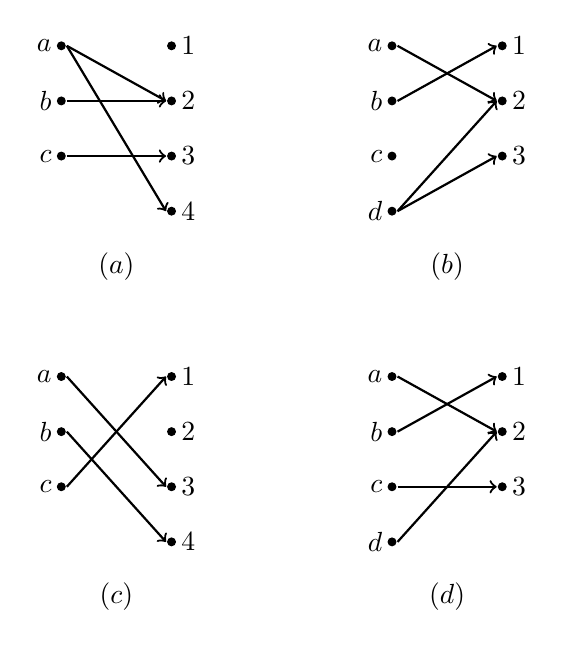
\begin{tikzpicture}[scale=0.7]
% Diagram (a)
\begin{scope}[shift={(0,0)}]
\filldraw (0,3) circle (2pt) node[left] {$a$};
\filldraw (0,2) circle (2pt) node[left] {$b$};
\filldraw (0,1) circle (2pt) node[left] {$c$};
\filldraw (2,3) circle (2pt) node[right] {$1$};
\filldraw (2,2) circle (2pt) node[right] {$2$};
\filldraw (2,1) circle (2pt) node[right] {$3$};
\filldraw (2,0) circle (2pt) node[right] {$4$};
\draw[->, thick] (0.1,3) -- (1.9,0);
\draw[->, thick] (0.1,3) -- (1.9,2);
\draw[->, thick] (0.1,2) -- (1.9,2);
\draw[->, thick] (0.1,1) -- (1.9,1);
\node at (1,-1) {$(a)$};
\end{scope}

% Diagram (b)
\begin{scope}[shift={(6,0)}]
\filldraw (0,3) circle (2pt) node[left] {$a$};
\filldraw (0,2) circle (2pt) node[left] {$b$};
\filldraw (0,1) circle (2pt) node[left] {$c$};
\filldraw (0,0) circle (2pt) node[left] {$d$};
\filldraw (2,3) circle (2pt) node[right] {$1$};
\filldraw (2,2) circle (2pt) node[right] {$2$};
\filldraw (2,1) circle (2pt) node[right] {$3$};
\draw[->, thick] (0.1,3) -- (1.9,2);
\draw[->, thick] (0.1,2) -- (1.9,3);
\draw[->, thick] (0.1,0) -- (1.9,2);
\draw[->, thick] (0.1,0) -- (1.9,1);
\node at (1,-1) {$(b)$};
\end{scope}

% Diagram (c)
\begin{scope}[shift={(0,-6)}]
\filldraw (0,3) circle (2pt) node[left] {$a$};
\filldraw (0,2) circle (2pt) node[left] {$b$};
\filldraw (0,1) circle (2pt) node[left] {$c$};
\filldraw (2,3) circle (2pt) node[right] {$1$};
\filldraw (2,2) circle (2pt) node[right] {$2$};
\filldraw (2,1) circle (2pt) node[right] {$3$};
\filldraw (2,0) circle (2pt) node[right] {$4$};
\draw[->, thick] (0.1,3) -- (1.9,1);
\draw[->, thick] (0.1,2) -- (1.9,0);
\draw[->, thick] (0.1,1) -- (1.9,3);
\node at (1,-1) {$(c)$};
\end{scope}

% Diagram (d)
\begin{scope}[shift={(6,-6)}]
\filldraw (0,3) circle (2pt) node[left] {$a$};
\filldraw (0,2) circle (2pt) node[left] {$b$};
\filldraw (0,1) circle (2pt) node[left] {$c$};
\filldraw (0,0) circle (2pt) node[left] {$d$};
\filldraw (2,3) circle (2pt) node[right] {$1$};
\filldraw (2,2) circle (2pt) node[right] {$2$};
\filldraw (2,1) circle (2pt) node[right] {$3$};
\draw[->, thick] (0.1,3) -- (1.9,2);
\draw[->, thick] (0.1,2) -- (1.9,3);
\draw[->, thick] (0.1,1) -- (1.9,1);
\draw[->, thick] (0.1,0) -- (1.9,2);
\node at (1,-1) {$(d)$};
\end{scope}
\end{tikzpicture}
\end{center}

\begin{enumerate}
\item Berdasarkan relasi-relasi diatas, manakah yang merupakan fungsi? Jelaskan jawaban Anda.
\item Sebutkan (satu-satu) anggota dari himpunan berikut.
\begin{align*}
A &= \{x|3 \leq x \leq 6, x \in \mathbb{Z}\} \\
B &= \{x|3 \leq x \leq 6, x \in \mathbb{R}\} \\
C &= \{x|3 < x < 6, x \in \mathbb{R}\}
\end{align*}
\end{enumerate}

\item Seorang pemburu bernama Kafka memiliki kontrak pekerjaan selama 10 minggu. Dia akan mengerjakan kontrak pekerjaan tersebut setiap hari dengan mengerjakan $n$ misi, dengan $n \in \mathbb{N}$ tetapi tidak melebihi 50 misi per harinya. Selidiki apakah terdapat barisan hari berturut-turut dimana Kafka mengerjakan tepat 87 misi. \textit{Hint}: Kafka minimal akan mengerjakan 1 misi per harinya.
\end{enumerate}

\end{document}